% ============================================================
%  fig_business_cycle.tex
%  景気循環（Cycle）と経済成長（Trend）の概念図
%
%  【単体コンパイル】
%    uplatex  fig_business_cycle.tex
%    dvipdfmx fig_business_cycle.dvi
%
%  【Beamer への組み込み】
%    プリアンブルに \usepackage{standalone} を追加し
%    \input{fig_business_cycle} で呼び出す
%
%  パネル構成:
%    (a) 上段: 実際の GDP とトレンド（対数スケール）
%    (b) 下段: 循環成分のみ（トレンドからの乖離）
%
%  使用マクロ:
%    T(x)  = 0.55x + 1.5            （トレンド）
%    Y(x)  = T(x) + 0.7*sin(1.8x + 0.3)  （GDP）
%    C(x)  = 0.7*sin(1.8x + 0.3)         （循環成分）
%
%  主要座標（数値は解析的に計算）:
%    Peak  : x = 0.706, 4.197, 7.688
%    Trough: x = 2.451, 5.942, 9.433
% ============================================================
\documentclass[tikz, dvipdfmx]{standalone}
\usepackage{tikz}
\usepackage{pgfplots}
\pgfplotsset{compat=1.18}
\usepgfplotslibrary{groupplots, fillbetween}
\usetikzlibrary{arrows.meta}

% ── カラー定義 ──────────────────────────────────────────────
\definecolor{gdpblue}{RGB}{30, 90, 180}
\definecolor{trendred}{RGB}{190, 40, 40}
\definecolor{expgreen}{RGB}{200, 230, 200}
\definecolor{recred}{RGB}{240, 200, 200}

\begin{document}
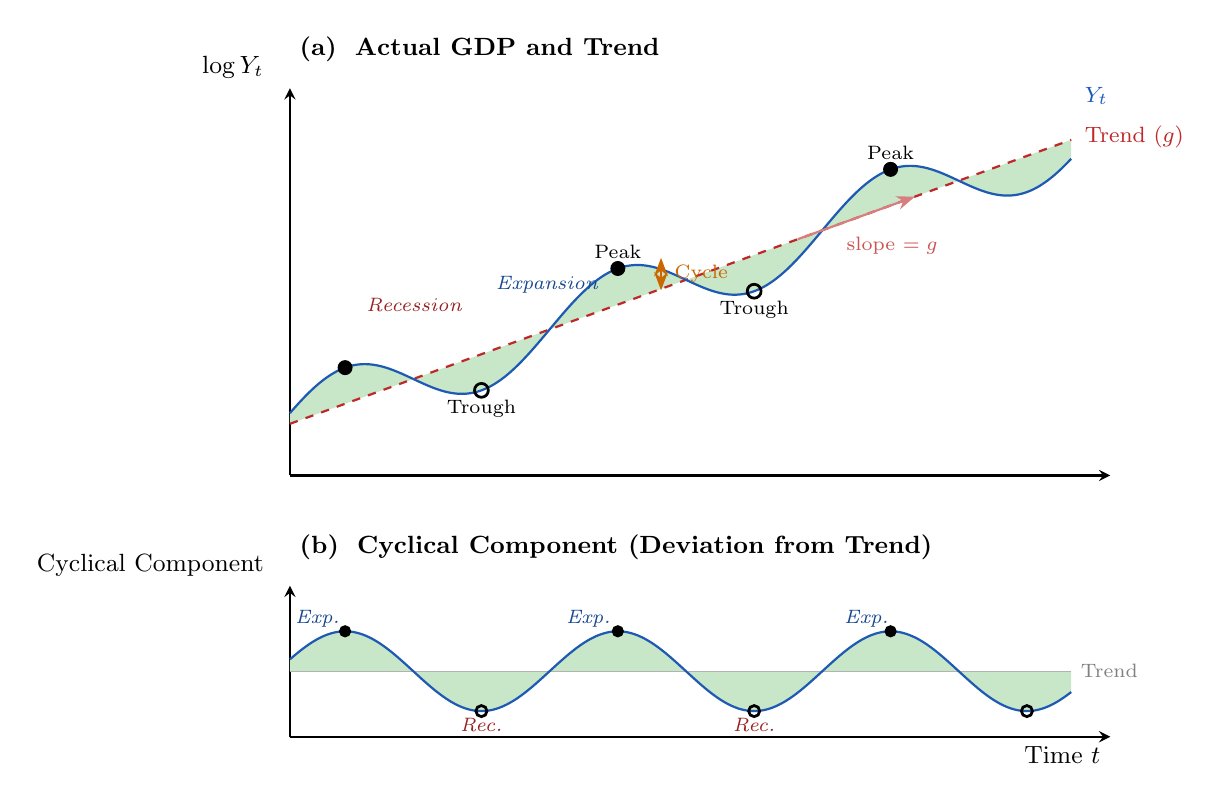
\begin{tikzpicture}

\begin{groupplot}[
  group style={
    group size  = 1 by 2,
    vertical sep= 14mm,
  },
  width  = 12cm,
  xmin   = 0,   xmax = 10.5,
  xtick  = \empty,
  ytick  = \empty,
  axis lines      = left,
  axis line style = {thick},
  clip            = false,
  every axis plot/.append style = {smooth},
]

% ════════════════════════════════════════════════════════════
%  上段パネル: 実際の GDP とトレンド
% ════════════════════════════════════════════════════════════
\nextgroupplot[
  height = 6.5cm,
  ymin   = 0.5, ymax = 8.0,
  ylabel = {$\log Y_t$},
  ylabel style = {
    rotate  = -90,
    at      = {(axis description cs: -0.02, 1.0)},
    anchor  = south east,
    font    = \small,
  },
  title  = {\textbf{(a)}\; Actual GDP and Trend},
  title style = {
    at     = {(axis description cs: 0, 1)},
    anchor = south west,
    font   = \small\bfseries,
  },
]

  %% ── fill between 用の透明パス ────────────────────────────
  \addplot[draw=none, name path=gdp_path,
    domain=0:10, samples=300]
    { 0.55*x + 1.5 + 0.7*sin(deg(1.8*x + 0.3)) };

  \addplot[draw=none, name path=trend_path,
    domain=0:10, samples=2]
    { 0.55*x + 1.5 };

  %% ── 拡張局面（GDP > Trend）と後退局面（GDP < Trend）の塗りつぶし
  %%    x=0 で sin(0.3)>0 → GDP>Trend → segment 0 = even → green
  \addplot fill between[
    of = gdp_path and trend_path,
    every even segment/.style = {fill=expgreen},   % 拡張: 緑
    every odd  segment/.style = {fill=recred},     % 後退: 赤
  ];

  %% ── トレンド線（赤破線） ─────────────────────────────────
  \addplot[trendred, thick, dashed, domain=0:10, samples=2]
    { 0.55*x + 1.5 };
  %% トレンドのラベル
  \node[right, font=\footnotesize, trendred]
    at (axis cs: 10.05, 7.05) {Trend ($g$)};

  %% ── GDP 線（青） ────────────────────────────────────────
  \addplot[gdpblue, thick, domain=0:10, samples=300]
    { 0.55*x + 1.5 + 0.7*sin(deg(1.8*x + 0.3)) };
  %% GDP のラベル
  \node[right, font=\footnotesize, gdpblue]
    at (axis cs: 10.05, 7.85) {$Y_t$};

  %% ── Peak マーカー（●） ──────────────────────────────────
  %%    座標: (0.706, 2.588), (4.197, 4.508), (7.688, 6.428)
  \addplot[only marks, mark=*, mark size=2.5pt,
    mark options={fill=black, draw=black}]
    coordinates { (0.706, 2.588) (4.197, 4.508) (7.688, 6.428) };
  \node[above, font=\scriptsize] at (axis cs: 4.197, 4.508) {Peak};
  \node[above, font=\scriptsize] at (axis cs: 7.688, 6.428) {Peak};

  %% ── Trough マーカー（○） ─────────────────────────────────
  %%    座標: (2.451, 2.148), (5.942, 4.068)
  \addplot[only marks, mark=o, mark size=2.5pt,
    mark options={fill=white, draw=black, line width=1pt}]
    coordinates { (2.451, 2.148) (5.942, 4.068) };
  \node[below, font=\scriptsize] at (axis cs: 2.451, 2.148) {Trough};
  \node[below, font=\scriptsize] at (axis cs: 5.942, 4.068) {Trough};

  %% ── 循環成分の振れ幅を示す両矢印 ────────────────────────
  %%    x = 4.7 付近（Peak x=4.197 の右）に描画
  %%    trend(4.7)  = 0.55*4.7+1.5 = 4.085
  %%    GDP(4.7)    ≈ 4.085 + 0.7*sin(8.76) ≈ 4.085 + 0.629 = 4.714
  \draw[<->, thick, orange!80!black, >=Stealth]
    (axis cs: 4.75, 4.085) -- (axis cs: 4.75, 4.714);
  \node[right, font=\scriptsize, orange!80!black]
    at (axis cs: 4.80, 4.40) {Cycle};

  %% ── 成長率を示す矢印（トレンドに沿った傾き） ─────────────
  \draw[->, thick, trendred!60, >=Stealth]
    (axis cs: 6.5, 5.075) -- (axis cs: 8.0, 5.900);
  \node[below right, font=\scriptsize, trendred!80]
    at (axis cs: 7.0, 5.3) {slope $= g$};

  %% ── Expansion / Recession テキスト ───────────────────────
  \node[font=\scriptsize, gdpblue!80!black]
    at (axis cs: 3.3, 4.2) {\textit{Expansion}};
  \node[font=\scriptsize, trendred!80!black]
    at (axis cs: 1.6, 3.8) {\textit{Recession}};


% ════════════════════════════════════════════════════════════
%  下段パネル: 循環成分のみ
% ════════════════════════════════════════════════════════════
\nextgroupplot[
  height = 3.5cm,
  ymin   = -1.15, ymax = 1.5,
  ylabel = {Cyclical Component},
  ylabel style = {
    rotate  = -90,
    at      = {(axis description cs: -0.02, 1.0)},
    anchor  = south east,
    font    = \small,
  },
  xlabel = {Time $t$},
  xlabel style = {
    at     = {(axis description cs: 1.0, 0)},
    anchor = north east,
    font   = \small,
  },
  title  = {\textbf{(b)}\; Cyclical Component (Deviation from Trend)},
  title style = {
    at     = {(axis description cs: 0, 1)},
    anchor = south west,
    font   = \small\bfseries,
  },
]

  %% ── fill between 用の透明パス ────────────────────────────
  \addplot[draw=none, name path=cycle_path,
    domain=0:10, samples=300]
    { 0.7*sin(deg(1.8*x + 0.3)) };
  \addplot[draw=none, name path=zero_path,
    domain=0:10]
    { 0 };

  %% ── 拡張（正）/ 後退（負）の塗りつぶし ──────────────────
  \addplot fill between[
    of = cycle_path and zero_path,
    every even segment/.style = {fill=expgreen},
    every odd  segment/.style = {fill=recred},
  ];

  %% ── ゼロ基準線 ───────────────────────────────────────────
  \addplot[gray!60, thin, domain=0:10] { 0 }
    node[right, font=\scriptsize, gray] {Trend};

  %% ── 循環成分の線 ─────────────────────────────────────────
  \addplot[gdpblue, thick, domain=0:10, samples=300]
    { 0.7*sin(deg(1.8*x + 0.3)) };

  %% ── Peak マーカー ────────────────────────────────────────
  \addplot[only marks, mark=*, mark size=2pt,
    mark options={fill=black, draw=black}]
    coordinates { (0.706, 0.7) (4.197, 0.7) (7.688, 0.7) };

  %% ── Trough マーカー ─────────────────────────────────────
  \addplot[only marks, mark=o, mark size=2pt,
    mark options={fill=white, draw=black, line width=1pt}]
    coordinates { (2.451, -0.7) (5.942, -0.7) (9.433, -0.7) };

  %% ── Expansion / Recession ラベル ─────────────────────────
  \node[font=\scriptsize, gdpblue!80!black]
    at (axis cs: 0.353, 0.92) {\textit{Exp.}};
  \node[font=\scriptsize, trendred!80!black]
    at (axis cs: 2.45,  -0.95) {\textit{Rec.}};
  \node[font=\scriptsize, gdpblue!80!black]
    at (axis cs: 3.82,  0.92) {\textit{Exp.}};
  \node[font=\scriptsize, trendred!80!black]
    at (axis cs: 5.942, -0.95) {\textit{Rec.}};
  \node[font=\scriptsize, gdpblue!80!black]
    at (axis cs: 7.38,  0.92) {\textit{Exp.}};

\end{groupplot}

\end{tikzpicture}
\end{document}
